\documentclass[landscape]{sciposter}
%\documentclass[landscape,draft]{sciposter}
\usepackage[]{graphicx}
\usepackage{amsmath,amsfonts,amssymb}
\usepackage{units}
\usepackage{authoraftertitle}
\usepackage[utf8]{inputenc}
\usepackage[T1]{fontenc}
\usepackage{charter}
\usepackage[expert]{mathdesign}
\usepackage{siunitx}
%\usepackage{fancyhdr}
%\usepackage{etoolbox}
%\renewcommand{\familydefault}{\rmdefault}

\usepackage{multicol}
\usepackage{url}

% Set the lengths of the pictures
\newlength{\customfigwidth}
\setlength{\customfigwidth}{16cm}

\newlength{\customfigheight}
\setlength{\customfigheight}{12cm}

\setlength{\belowdisplayskip}{10pt} \setlength{\belowdisplayshortskip}{10pt}
\setlength{\abovedisplayskip}{10pt} \setlength{\abovedisplayshortskip}{10pt}
\setlength{\columnseprule}{4pt}
\setlength{\multicolsep}{6.0pt plus 2.0pt minus 1.5pt}% 50% of original values
\setlength\columnsep{40pt}% 50% of original values

\newcommand{\eqnote}[1]{{\scriptsize#1}}


\usepackage[font={large,it}]{caption}
\usepackage[protrusion=true,expansion=true]{microtype}

% Convenience functions
\newcommand{\pfrac}[2]
        {\frac{\partial #1}{\partial #2}}       % partial 1 /partial 2 
\newcommand{\ket}[1]
        {\left | \, #1 \right \rangle}          % bra-ket notation
\newcommand{\abs}[1]{
        \left\vert #1 \right\vert}		% vert bars for averages
\newcommand{\norm}[1]
        {\left\Vert #1 \right\Vert}             % taller vert bars for the norm
\newcommand{\evalat}[1]
        {\left. #1 \right \vert}        % ex. evaluating the int. at its limits
\newcommand{\set}[1]
        {\left\{ #1 \right\}}           % squigle brackets for sets
\newcommand{\avg}[1]
        {\left< #1 \right>}		% angle brackets for averages < >
\newcommand{\paren}[1]
        {\left( #1 \right)}		% grows parentheses () 
\newcommand{\brackets}[1]
        {\left[ #1 \right]}		% grows square brackets []
\newcommand{\braces}[1]
        {\left \{ #1 \right \}}         % grows curly brackets {}
\newcommand{\piecewisebrace}[1]
        {\left \{ #1 \right .}          % piecewisebrace

% Shorthand with proper spacing
\newcommand{\viz}{viz.\ }
\newcommand{\ie}{i.e.\ }
\newcommand{\eg}{e.g.\ }
\newcommand{\cf}{c.f.\ }

% Chemical formula
\newcommand{\chem}[1]{\ensuremath{\mathrm{#1}}} 

% New math operators
\DeclareMathOperator*{\minor}{minor\,}
\DeclareMathOperator*{\sgn}{\mathbf{sgn}\, }
\DeclareMathOperator*{\rootof}{RootOf\,}

% Vector notation
\newcommand{\mathvect}[1]{\boldsymbol{#1}}
\newcommand{\vect}[1]{\mathbf{#1}}

% Differential used at the end of an integral
\newcommand*\diff{\mathop{}\!\mathrm{d}}
\newcommand{\integral}[2]{\int #1\diff#2}


% Equation placeholders
\newcommand{\SPHYvals}{%
  Y_{\ell m}^{*} ( \hat{\vect{r}}_i ) 
  Y_{\ell m}     ( \hat{\vect{r}} ) 
}

\newcommand{\SPHsumterms}{%
    \sum_{\ell=0}^\infty \sum_{m=-\ell}^{\ell} %
}

\newcommand{\SPHsum}[1]{%
  \SPHsumterms
  #1
  \SPHYvals
}

\newcommand{\normdiff}[1]{%
  \norm{ \vect{#1} - \vect{#1}_i}
}

\newcommand{\ViralInteractionPot}{\Phi_{12}}
\newcommand{\transpose}[1]{^{\intercal}}

\newcommand{\sphericalBesselIN}{ i }
\newcommand{\sphericalBesselKN}{ k }
\newcommand{\knownPHI}{\Psi}
\newcommand{\macroPHI}{\Phi}

\newcommand{\pka}{\text{pKa}}
\newcommand{\pH}{\text{pH}}
\newcommand{\LMAX}{\ell_{\text{MAX}}}

\newcommand{\effChargeLocations}{\vect{r}_1, \vect{r}_2, \ldots, \vect{r}_N}
\newcommand{\fittingACCeffective}{\chi}
\newcommand{\debyehukel}{Debye-H\"{u}ckel }

%\definecolor{BoxCol}{rgb}{.93531, .93531, .93531}
%\definecolor{palered}{RGB}{255,182,182}


\newcommand{\titlefont}[1]{%
  {%
  \usefont{T1}{bch}{b}{n}%
    \selectfont%
    #1%
  }%
  \normalfont%
}

\newcommand{\at}{\makeatletter\titlefont{@}\makeatother}


\author{Travis Hoppe, Robert Best}
\email{hoppeta@mail.nih.gov}
\institute{National Institutes of Health, National Institute of Diabetes and Digestive and Kidney Diseases}
\conference{\titlefont{\large Biophysical Society Meeting 2016, Los Angeles CA}}

\renewcommand{\sectionsize}{%
  \usefont{T1}{bch}{b}{n}%
  \scshape%
  \bfseries%
  \large
  \selectfont%
}
 
\begin{document}

% Custom footer
\renewcommand{\footlogo}{%
  \resizebox{2\logowidth}{!}{%
    
\includegraphics[height = 1cm]{logos/NIDDK_logo.pdf}%
    \hspace{1em}
    
\includegraphics[height = 1cm]{logos/dhhs_logo.pdf}%
    \hspace{1em}
    
\includegraphics[height = 1cm]{logos/NIH_Logo.pdf}
  }
}

% Custom title
%\maketitle
\resizebox{\textwidth}{!}{
  \begin{tabular}{ p{.6\textwidth} r }
    \titlefont{\Huge  Enhancing the Coevolutionary Signal }  &
    \titlefont{\Large \MyAuthor} \\
    %& 
    \titlefont{\Large via machine learning}&
    %\includegraphics[height = 1cm]{mail.png}
    \texttt{hoppeta}{\bfseries \at}\texttt{mail.nih.gov}
    %&
  \end{tabular}
}
\vspace{1cm}


\begin{multicols}{3}

\section*{Abstract}
Analysis of coevolutionary relationships between residue pairs in the sequences of folded proteins can yield information on which residues interact in the folded state, and hence produce a contact map based only on sequence information. 
The distribution of contacts in folded proteins is far from random, as evident from looking at any contact map. 
Therefore, it should be possible to use information from neighboring contacts in order to strengthen the predictive power of coevolutionary analysis. 
Here, we show that application of a machine-learning algorithm to contact maps from analysis of evolutionary couplings significantly improves the precision of the derived contact map with a sacrifice in sensitivity, so that many more contacts can be predicted with confidence. 

\vfill
\columnbreak

\section*{Hypothesis / Motivation}

In the sequence to structure prediction problem, it has been particularly fruitful to incorporate coevolutionary data.
The assumption is that co-mutating residues in multiple sequence alignment have a higher probability of being in contact in the three-dimensional structure.
\vfill
We concentrate on improving one of these models, GREMLIN\cite{kamisetty2013assessing}, though the methods would work on similar schemes like DCA and PSICOV.
In GREMLIN the top $L$ residue pairs are chosen from a coevolutionary scoring matrix. 
This works well for low values of $L$ but the signal-to-noise ratio drowns out the weaker contacts.
\vfill
We propose a straight-forward machine learning scheme to infer a contact from the \emph{local} score pattern with the physically motivated hypothesis that the presence of a high local scores are an indicator of a contact.

\vfill
\columnbreak

\section*{Coevolutionary Analysis: GREMLIN\cite{kamisetty2013assessing}}

GREMLIN optimizes the pseudolikelihood  of a maximum entropy model that matches the observed single and pair frequencies from a multiple sequence alignment:

$$ P(v,w | D) = \sum_{n=1}^N \sum_{i=1}^L \log P (x_i^n | x_{i'}^n, v, w)$$

$$ P (x_i^n | x_{i'}^n, v, w) = \frac{1}{Z_i} \exp \left ( v_i(x_i^n) + \sum_{j=1,j \neq i}^L w_{ij}(x_i^n,x_j^n) \right )$$

$v_i$ encodes individual propensity of each amino acid at position $i$ $w_{ij}$ statistical coupling of amino acid propensities between positions $i,j$. 
This formulation models conditional distribution of the original joint distribution instead of the joint distribution itself. 

\end{multicols}

\begin{multicols}{3}

\section*{Methods}

\begin{itemize}
\setlength\itemsep{0.8em}
\item 150 globular proteins (50-275 residues each) were selected from set of non-homologous proteins covering diverse motifs and structures.
\item Proteins were aligned using HHBLITS.
\item Alignments were scored using GREMLIN.
\item Scores were reduced from the original $(N,N,21,21)$ tensor by dropping gaps, taking the Frobenius norm and applying the Average Product Correlation (APC).
\item Using a 4-fold cross-validated scheme, ``images'' of 5x5 were taken from the training set of GREMLIN scores to predict if a true native contact was given at the center.
\item An extremely random forest (RF) was trained over the images.
\item Contact maps for a given cutoff were predicted from both the GREMLIN and RF models.
\item Coarse-grained molecular dynamics simulations were performed with each contact map to test folding.
\end{itemize}

%Protein dataset taken from PSICOV %.\cite{jones2012psicov}.

\vfill \columnbreak

\section*{Improved Contact Map Prediction}

\begin{figure}
    \center 
    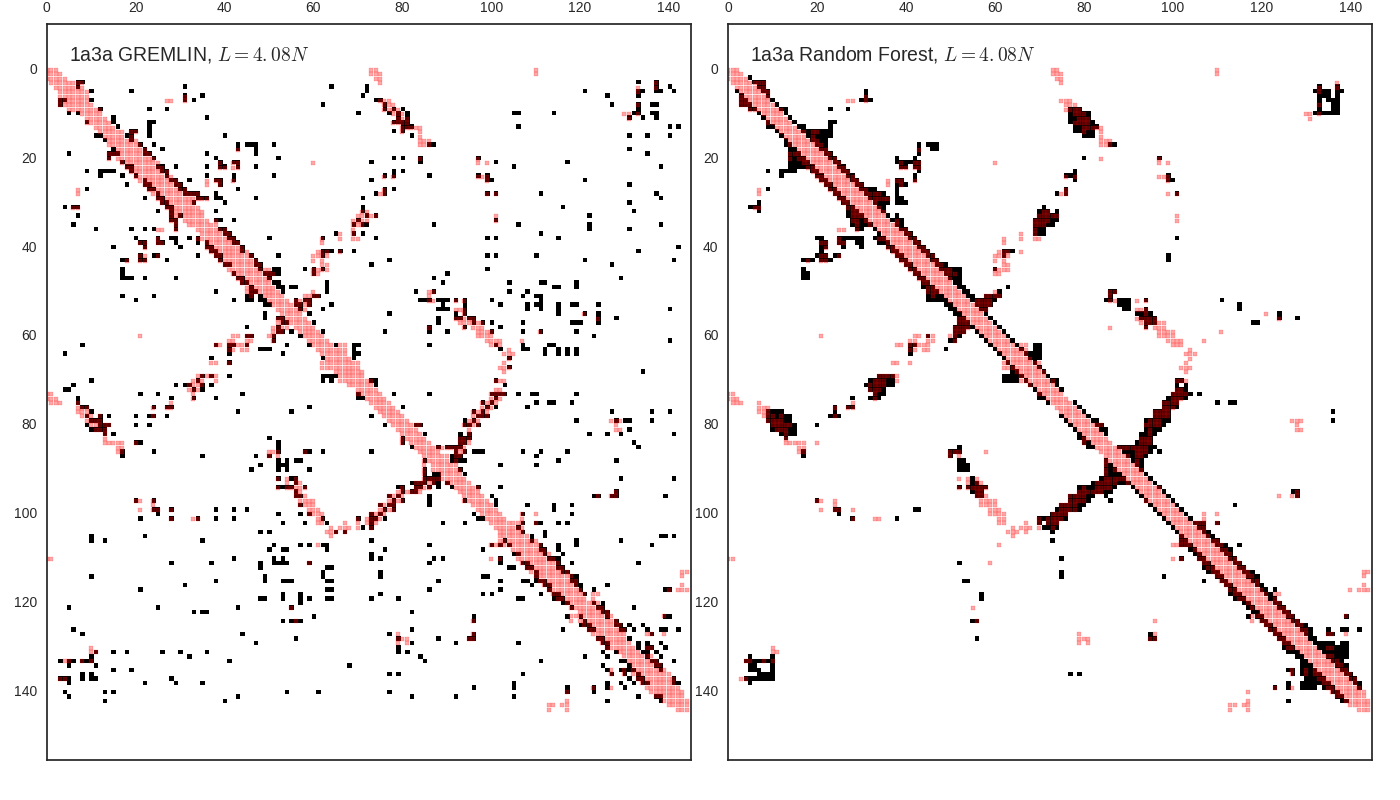
\includegraphics[height=1.25\customfigheight]{figures/1a3a_cmp.png}%
\caption{
Both: contact map of protein 1a31 (IIA Mannitol from E. Coli) in red;
Left: original GREMLIN scoring method on in black; 
Right: improved RF in black.

Using the traditional scoring method, false positives appear uniformly randomly across the contact pairs, 
while the RF method is more precise  by utilizing local information.
}
\end{figure}

\vfill \columnbreak

\section*{ROC Curve}
\begin{figure}
    \center 
    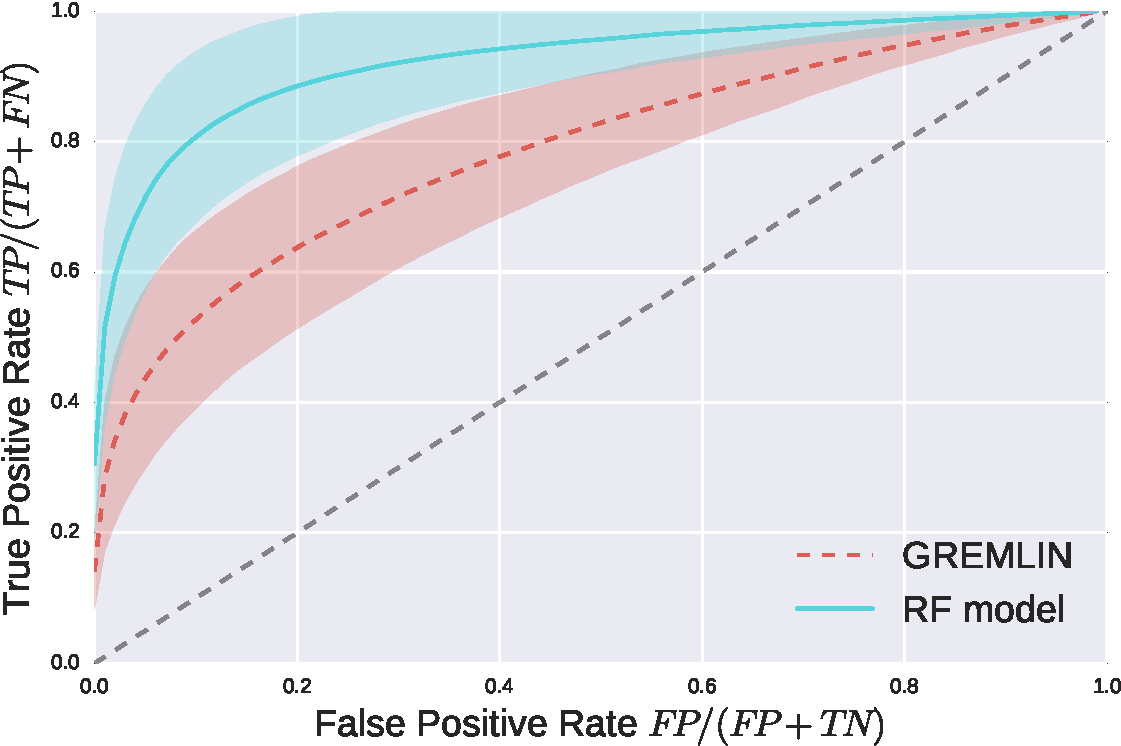
\includegraphics[height=\customfigheight]{figures/GREMLIN_RF_ROC-crop.pdf}%
    \hfill%
    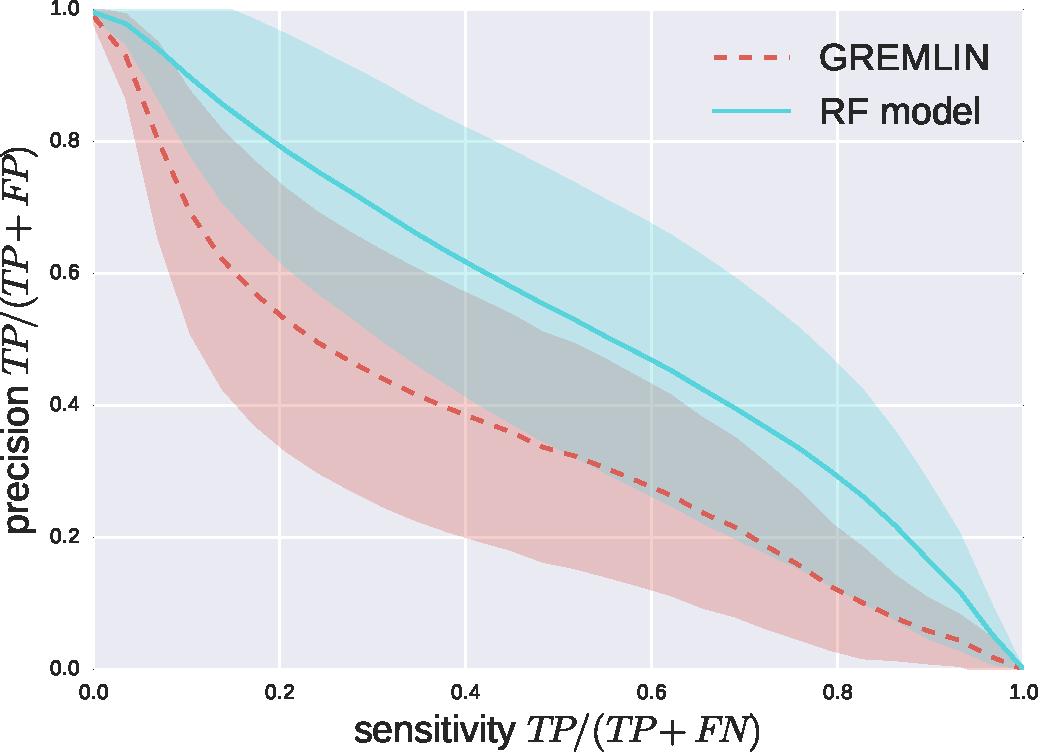
\includegraphics[height=\customfigheight]{figures/GREMLIN_RF_Acc_Pre-crop.pdf}%
\caption{%
Left: Receiver operating curve for GREMLIN and RF models; Right: same for sensitivity vs. precision. 
For all values of the sensitivity, RF-GREMLIN outperforms the traditional GREMLIN by choosing more correct contacts.
}

\end{figure}

\end{multicols}

\begin{multicols}{3}

\section*{Contact improvement is localized}

\begin{figure}
    \center 
    \hfill%
    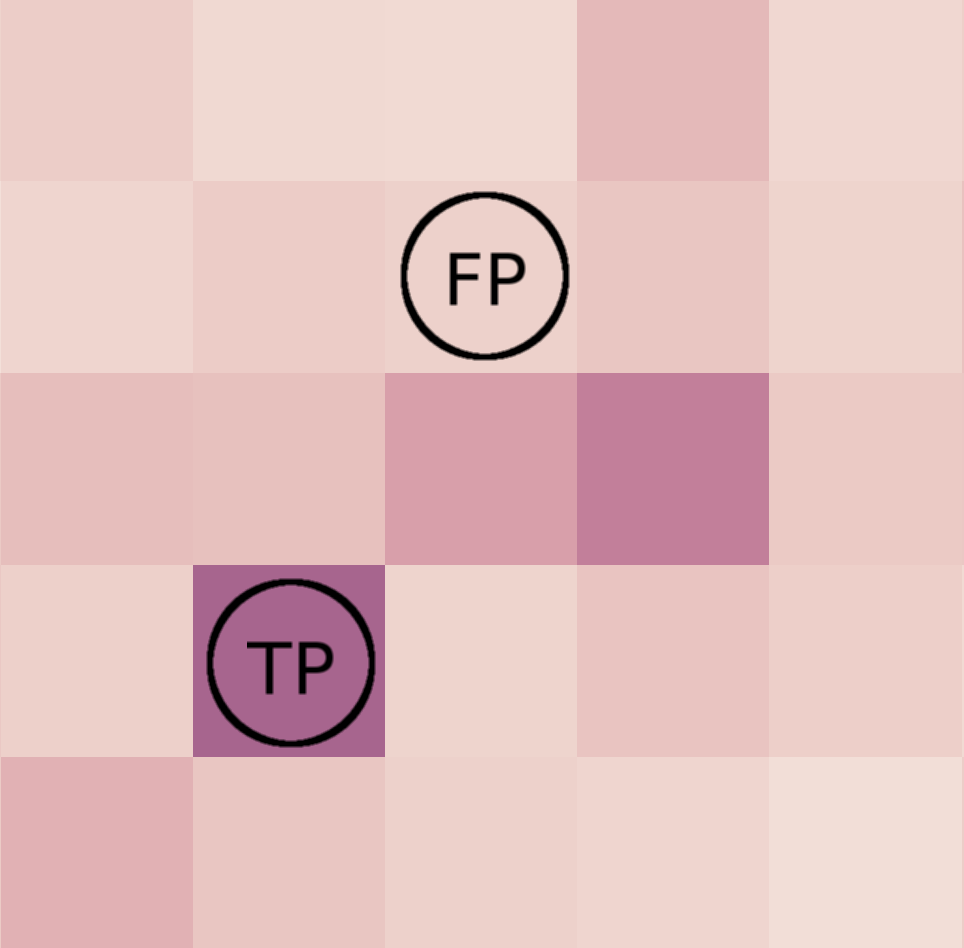
\includegraphics[height=1.2\customfigheight]{figures/local_structure_distance.png}%   
    \hfill%
    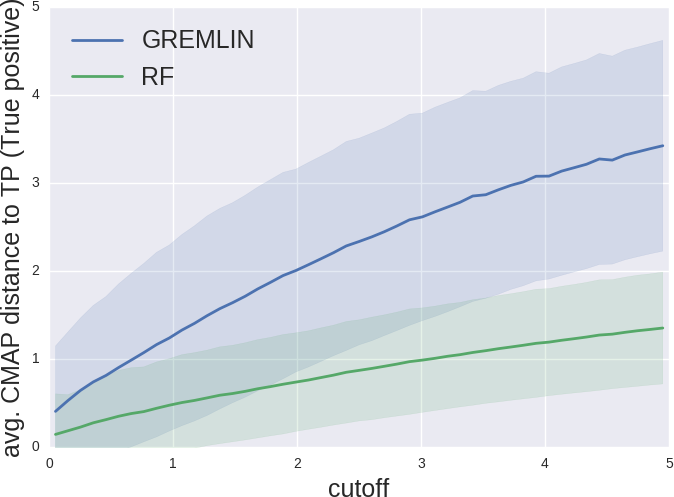
\includegraphics[height=1.2\customfigheight]{figures/FP_distance.png}%
    \hfill%
    \hspace{0em}

\caption{%
Both methods give false positive (FP), but the predictions by the RF were closer to the true positives (TP) in contact map space.
We measured the average city-block (L1-norm) distance from each FP to the nearest TP and averaged over all proteins contact maps predicted. 
Left: diagrammatic illustration of a FP to a TP, showing a distance of three. Right: Averaged L1 distance for all FPs to TPs across the dataset.
}
\end{figure}

\vfill \columnbreak

\section*{Folding simulations}
\begin{figure}
    \center 
    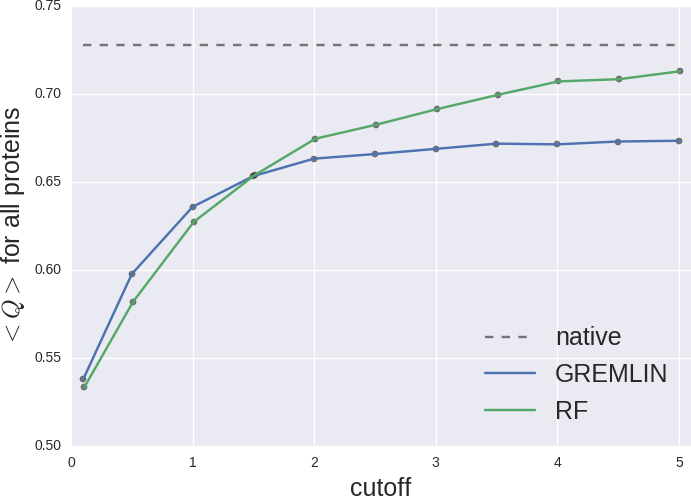
\includegraphics[height=1.25\customfigheight]{figures/folding/Q_avg.png}

\caption{
To test the efficacy of the contact maps as a tool to predict the native fold of a protein (without any other prior knowledge) we employed a coarse-grained molecular-dynamics simulation. 
Each residue was modeled by a single $C_\alpha$ atom with a standard backbone potential and an attractive component if two residues were predicted to be in contact.
The fraction of true native contacts formed after a short folding simulation, $Q$, are plotted.
}
\end{figure}


\vfill \columnbreak

\section*{Feature selection}

\begin{figure}
    \center 
    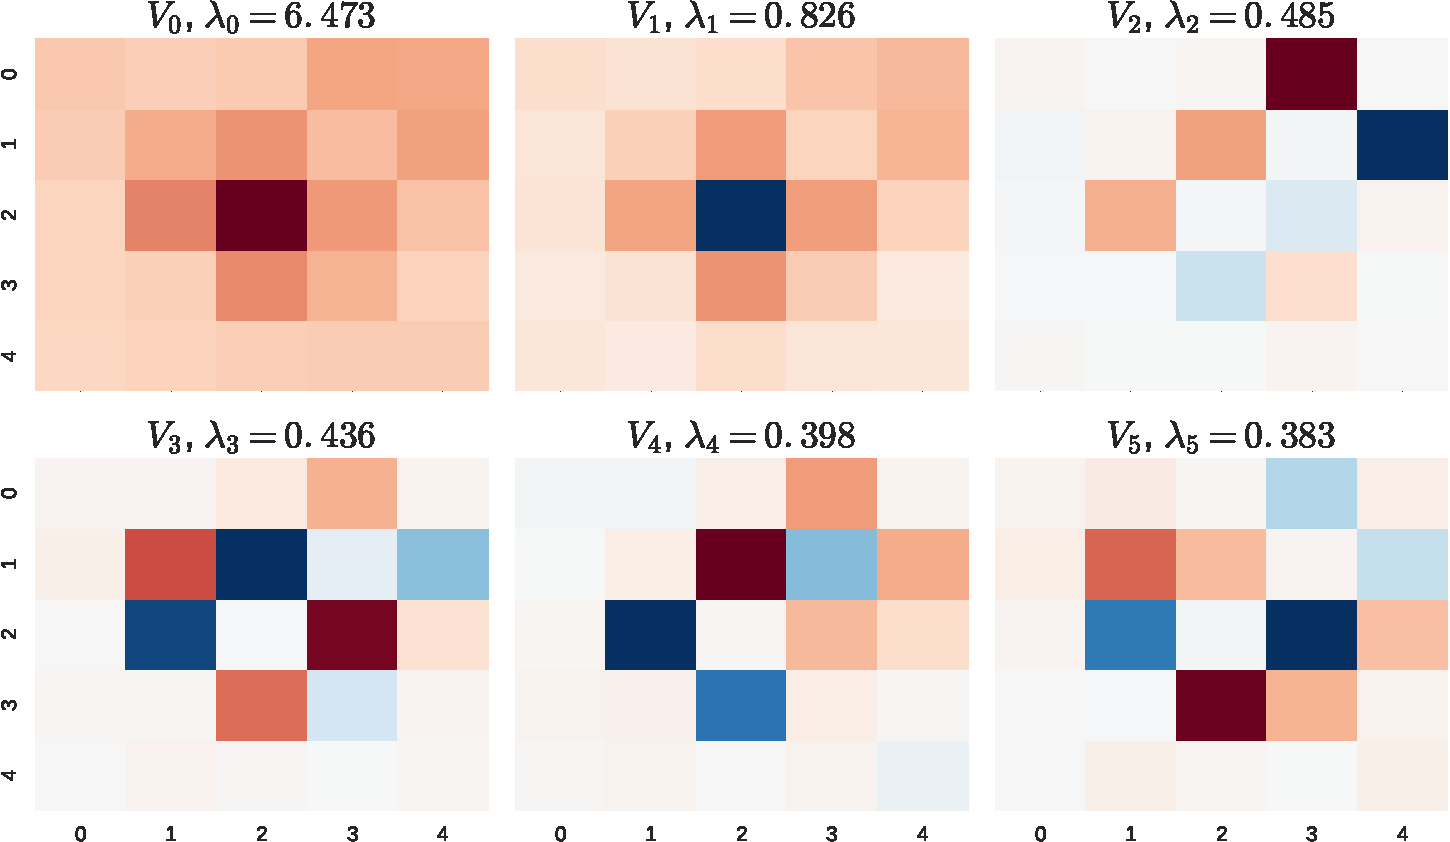
\includegraphics[width=1.25\customfigwidth]{figures/avg_features-crop.pdf}%
\caption{
To illustrate feature selection of the model, we perform singular value decomposition of terminal leaf nodes from the random forests. The dominant features ($V_1, V_2$) are roughly described by a Gaussian kernel and the difference between the center and the outlying values.
}
\end{figure}

%\renewcommand{\refname}{} 
\bibliographystyle{unsrt}
%\bibliographystyle{plain}  % enter bibligraphy as usual, with or without using
\small                     
\bibliography{bib/CMAP.bib} 

%\renewcommand{\refname}{xxx} 
%\begin{sectionbox}{}  
% changes section heading over bibliography

%\bibliography{../bib/AnisoChargeFits.bib}
%\end{sectionbox}

\end{multicols}

 
\end{document}
